\chapter{系统架构}
\oneline{安路 FPGA 双板实时视频系统:相机主板(PH1P35)把 SC500CS 图像经自研 ISP
处理后以千兆 UDP 推流;PC 上位机收图并网络控制曝光/白平衡/模式;显示子板
(EG4D20)接收同一路码流,经帧重组、DDR 三缓冲后输出 HDMI 720p60 实时回显。}

\section{系统概览}

系统由一块相机主板、一块显示子板与 PC 上位机构成(图~\ref{fig:system})。主板
(MLKPAI-F02,安路 PH1P35)完成图像采集、ISP 处理与千兆 UDP 推流,具有两个以太网
口:ETHA 连接 PC 上位机(收图与控制),ETHB 为镜像输出口,输出与 ETHA 完全相同的
RGMII 发送流。显示子板(MLKPAI-F01,EG4D20)从 ETHB 直连网线接收码流,完成协议
解析、帧重组与三缓冲后以 HDMI 720p60 输出到显示器——它是纯接收显示设备,无命令
通路、零参数调节。PC 上位机(Python GUI)经 UDP 6000 收图预览、UDP 6001 下发
曝光/白平衡/模式命令、UDP 6002 接收状态与应答。

\begin{figure}[H]\centering
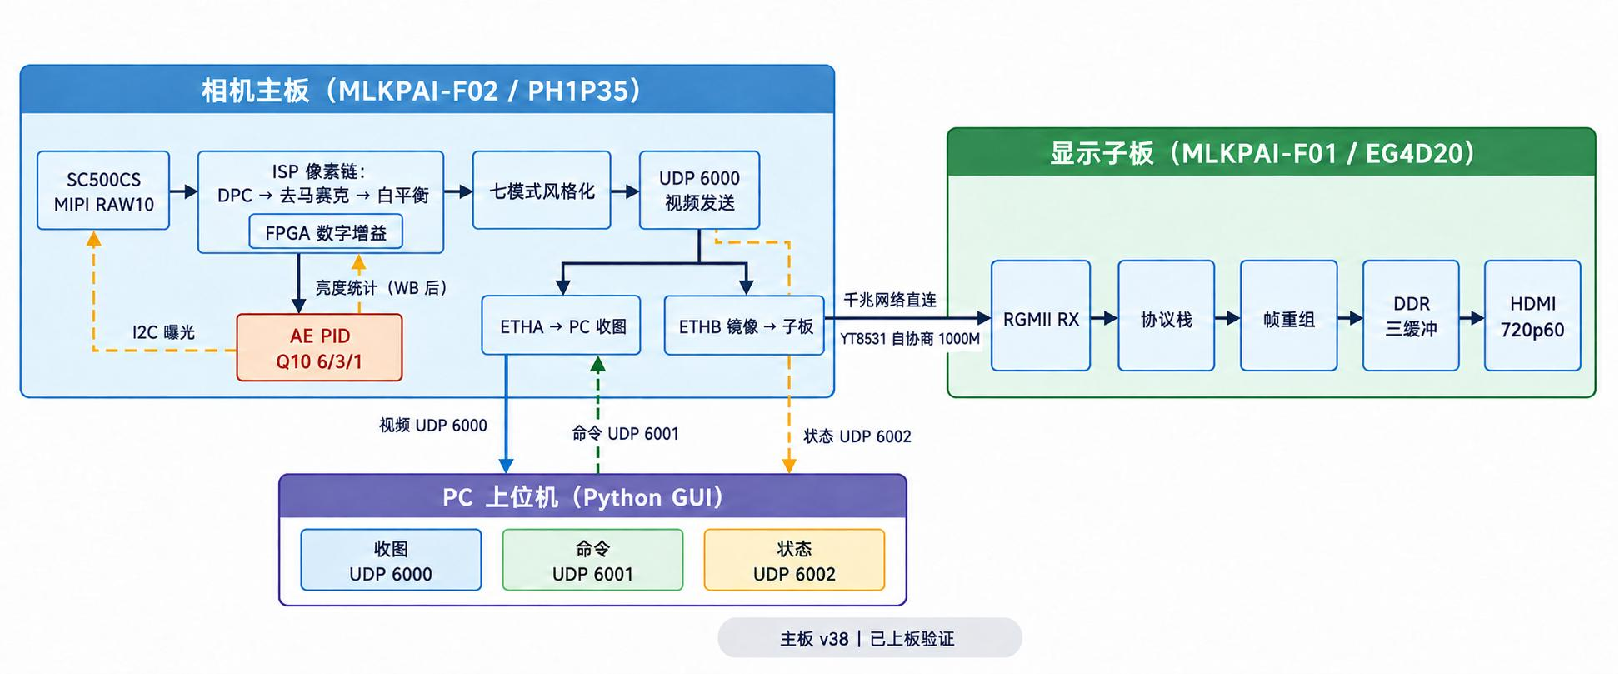
\includegraphics[width=\textwidth]{figs/fig_system.pdf}
\caption{双板系统总览:相机主板、显示子板与 PC 上位机}
\label{fig:system}
\end{figure}

两路显示并行:PC 端预览(ETHA)与子板 HDMI 回显(ETHB)。主板本地 DDR/DSI
显示支路已在 v30 裁剪,7 寸屏背光关闭;网络镜像和相机处理链不依赖该支路。子板
偶发丢包由帧重组器容忍:不超过 4 包的缺口采用最后有效像素冻结延展,更大缺口
跟踪并丢弃至下一帧头,无需重传。主板当前软件基线为 v38
(PID Q10 系数 6/3/1),子板为 v28;当前源码已完成仿真、综合、布线与上板验证。

\section{关键技术指标}

系统的关键技术指标汇总如下表。

\begin{table}[H]\centering\small
\caption{系统关键技术指标}
\begin{tabular}{>{\bfseries}l p{11.2cm}}
\toprule
图像规格 & 1280$\times$720 RGB888;主板采集与推流 30\,fps,子板 HDMI 输出 60\,Hz \\
视频链路 & UDP 6000,每帧 1920 包 $\times$ 1440 字节(480 像素/包),包头 6 字节
(帧序号/格式/4 字节大端偏移);线速约 697\,Mbps(千兆链路必须) \\
命令/状态链路 & UDP 6001 命令(广播,魔数校验);UDP 6002 状态与应答包 \\
网络约定 & 板卡 192.168.1.66;PC 192.168.1.100/24;子板本地 IP 设为流的
目的地址,PC 控制侧不占用该地址 \\
主板器件 & 安路 PH1P35(MLKPAI-F02)+ SC500CS 摄像头模组 + YT8531 千兆 PHY
$\times$ 2 \\
子板器件 & 安路 EG4D20(MLKPAI-F01,EG4D20EG176)+ YT8531 千兆 PHY + 合封
DDR1 16MB \\
板间链路 & 千兆网线直连,两端 YT8531 自协商 1000M \\
上位机 & Python GUI:收图/预览/存帧,曝光、增益、白平衡四模式、算法模式切换 \\
运行验证 & 历史主板七模式 + AE/AWB 连续运行 300\,s,平均 29.965\,fps、
完整率 100\%,无视频流/I2C 错误;该定量板测早于 v38。v38 源码已上板验证,
仿真/综合/布线结果如下:
Setup WNS +0.119\,ns、Hold WNS +0.020\,ns、TNS 均为 0,Slice 10944/21216
(51.58\%)。本文未将早期板测帧率数据误记为 v38 数据。子板全分辨率真机工况仿真(1920 包/帧 $\times$ 11 帧)
逐字节比对通过,上板 HDMI 显示正常 \\
\bottomrule
\end{tabular}
\end{table}

\section{文档组织}

本技术文档按"系统—主板—子板—应用"组织:第 2 章讲主板相机工程的数据通路
(采集解包 $\to$ ISP $\to$ 推流);第 3 章讲 ISP 与图像算法(像素处理链、DPC、
去马赛克、色彩校正与 AWB/AE 两个 3A 闭环、七种风格化模式);第 4 章讲命令通路
与运行时控制(命令解析、I2C 执行通道、手动/自动语义);第 5 章
讲子板 HDMI 回显工程(RGMII 接收、协议栈、帧重组器、DDR 三缓冲、显示输出);
第 6 章讲血细胞形态学检测应用设计。各章自成体系,交叉处以"见第 X 章"互引。

\section{仓库结构}

\begingroup\scriptsize
\begin{verbatim}
CameraVideoPath-on-fpga/
├── README.md                    本文档:系统拓扑、双板工程入口、验证摘要
├── 08_csi_dsi_cs500_7cun/       主板相机工程:MIPI 接收、ISP、风格化、UDP 发送、
│                                上位机脚本、TD 工程、发布说明
├── HDMI_OUT/                    子板 HDMI 回显工程:
│   ├── uisrc/01_rtl/            cvp_hdmi_top(顶层) cvp_rx_assemble(帧重组)
│   │                            rgmii_cdc(跨时钟域) osd_anlogic_logo(OSD)
│   ├── uisrc/03_ip/             复用例程 IP:UDP 协议栈/FDMA/DDR1/VTC/HDMI TX
│   ├── uisrc/04_pin/            引脚与时序约束(pin.adc / timing.sdc)
│   ├── tools/sim/               ModelSim 全链路仿真(Python 向量注入+记分板回归)
│   └── doc/                     架构文档与调试交接
├── releases/                    各版本比特流与发布记录
└── 技术文档/                    本技术文档系列
\end{verbatim}
\endgroup

{\small\sloppy\textbf{说明:}\ 主板与子板工程分别对应独立 TD 工程
(\texttt{camera\_to\_dsi\_display.al} 与 \texttt{HDMI\_OUT.al}),均以 PROGRAM\_SRAM
方式加载(SRAM 断电丢失)。子板复用厂商例程的协议栈、FDMA、DDR 与 HDMI 发送 IP,
其中仅 \texttt{uimac\_rx.v} 有一处有意修改(广播 IP 帧放行),从例程目录重新拷贝
时必须保留该补丁。}

\section{设计原则}

全系统贯彻四条原则。其一,\textbf{流式处理}:主板 ISP 与子板重组器均为无反压流式
流水,常数延迟、按拍处理。其二,\textbf{接口标准化}:主板内部以 128\,bit 公共像素
流接口(CVP\_PIXEL\_V1,含坐标/帧身份/模式号元数据)贯穿算法挂接点,即插即用。
其三,\textbf{验证闭环}:v38 的 42 项 RTL、两组网络包校验、38 项 Python
回归与 460 帧视频链路模型通过;v29 资源优化的 22 项回归(含新旧实现同激励逐位差分对照)、子板 8 场景记分板
与全分辨率逐字节比对等仿真均通过,当前源码已完成上板验证。其四,\textbf{约束显式化}:两板
的时钟组、采样相位与带宽预算全部显式声明并留余量(子板 DDR1 带宽占峰值 55\%)。
